%%%%%%%%%%%%%%%%%%%%%%%%%%%%%%%%%%%%%%%%%%%%%%%%%%%%%%%%%%%%%%%%%%%%%%%%%%%
% Assignment 2.1: Creating a histogram by hand
%%%%%%%%%%%%%%%%%%%%%%%%%%%%%%%%%%%%%%%%%%%%%%%%%%%%%%%%%%%%%%%%%%%%%%%%%%%

\handassignment{Assignment 2.1: Creating a histogram by hand}

Suppose that you have the following set of numbers: \\

\begin{center}
\hspace{0.3cm}1.5\hspace{0.3cm}5.5\hspace{0.3cm}1.7\hspace{0.3cm}7.2\hspace{0.3cm}1.2\hspace{0.3cm}7.9\hspace{0.3cm}1.4\hspace{0.3cm}3.6\hspace{0.3cm}3.1\hspace{0.3cm}3.8\hspace{0.3cm}5.9\hspace{0.3cm}3.6\hspace{0.3cm}5.1\hspace{0.3cm}3.2\hspace{0.3cm}7.1
\end{center}

\question{
    2.1 a
}{
    For each of the ranges given below, find out their \concept{frequency} in the data above.
}

\emptyanswerbox{
    2.1a
}{
    \begin{center}
    \begin{tabular}{|c|c|c|c|}
    \hline
    0 to 2 & 2 to 4 & 4 to 6 & 6 to 8 \tstrut\bstrut\\
    \hline
    & & & \\
    Frequency:\hspace*{2pt}\rule{0.8cm}{0.4pt}  & Frequency:\hspace*{2pt}\rule{0.8cm}{0.4pt} & Frequency:\hspace*{2pt}\rule{0.8cm}{0.4pt} & Frequency:\hspace*{2pt}\rule{0.8cm}{0.4pt} \bstrut\\
    \hline
    \end{tabular}
    \end{center}
}

\question{
    2.1 b
}{
    Draw the histogram for these data by hand. The name of the \textit{x-axis} should represent the range of values, and the name of the \textit{y-axis} should represent the \concept{frequency} of the values that fall in the ranges of assignment 2.1a.
}

\emptyanswerbox{
    2.1 b
}{
    \vspace*{-0.5cm}
    \begin{center}
    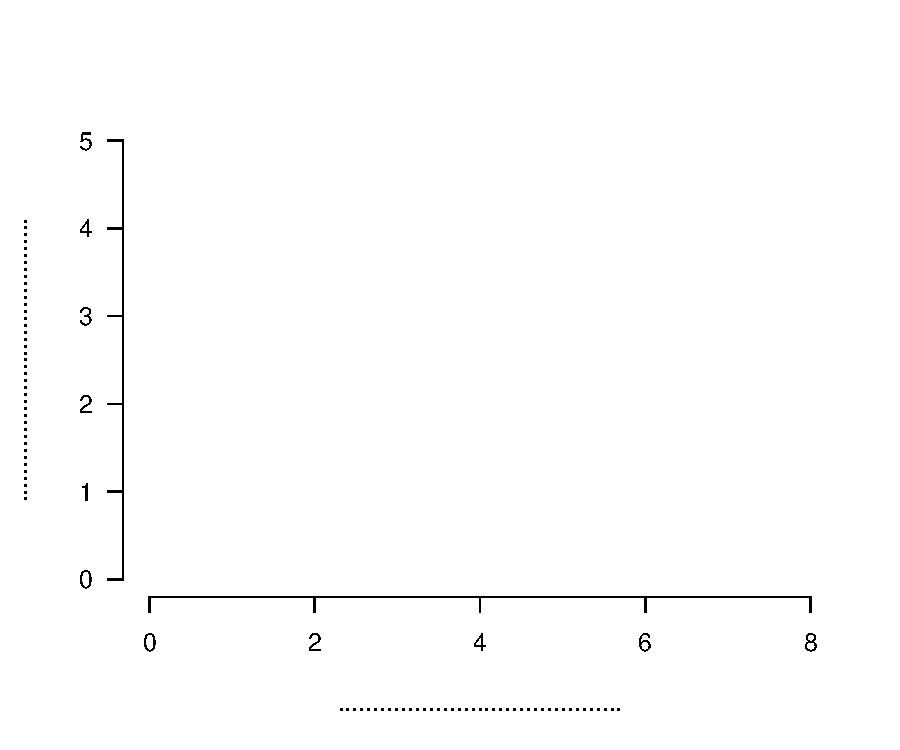
\includegraphics[height = 7cm]{Files/Images/emptyHistogram.pdf}
    \end{center}
}

\clearpage % Page break